\chapter{Исследовательская часть}

\section{Технические характеристики}

Технические характеристики устройства, на котором выполнялось тестирование:

\begin{itemize}
	\item операционная система: Windows 10;
	\item оперативная память: 16 Гб;
	\item процессор: Intel® Core™ i5-8259U;
	\item количество ядер: 4;
	\item количество логических процессоров: 8.
\end{itemize}

Во время тестирования ноутбук был включен в сеть питания и нагружен только встроенными приложениями окружения и системой тестирования.

\section{Пример работы программы}
На рисунке \ref{fig:work_example} приведен пример работы программы.
\clearpage
\begin{figure}[h!]
	
	\centering{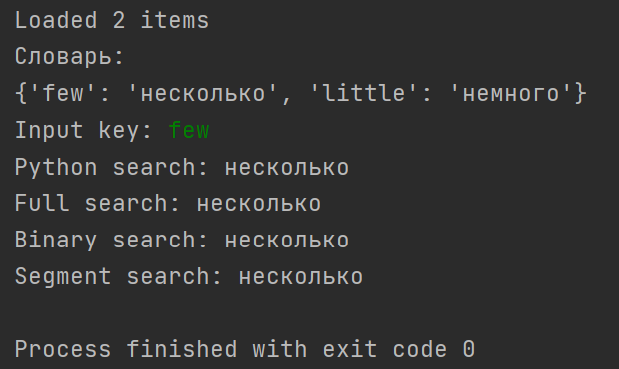
\includegraphics[scale=1]{inc/img/work_example.png}}
	
	\caption{Пример работы программы}
	
	\label{fig:work_example}
	
\end{figure}


\section{Сравнение трудоемкостей реализаций}
полный перебор
Трудоёмкость алгоритма зависит от того, присутствует ли искомый ключ в словаре. Если такого ключа нет, то она определяется количеством ключей в словаре, если есть -- его удаленностью от начала массива ключей.

Пусть алгоритм нашёл элемент на первом сравнении (лучший случай), тогда будет затрачено $k_0 + k_1$ операций, на втором - $k_0 + 2 \cdot k_1$, на последнем (худший случай) - $k_0 + N \cdot k_1$. Если ключа нет в массиве ключей, то мы сможем понять это, только перебрав все ключи, таким образом трудоёмкость такого случая равно трудоёмкости случая с ключом на последней позиции. Средняя трудоёмкость может быть рассчитана как математическое ожидание по формуле (\ref{for:brute}), где $\Omega$ -- множество всех возможных случаев.

\begin{equation}
	\label{for:brute}
	\begin{aligned}
		\sum\limits_{i \in \Omega} p_i \cdot f_i = & (k_0 + k_1) \cdot \frac{1}{N + 1} + (k_0 + 2 \cdot k_1) \cdot \frac{1}{N+1} +\\
		& + (k_0 + 3 \cdot k_1) \cdot \frac{1}{N + 1} + (k_0 + Nk_1)\frac{1}{N + 1} + (k_0 + N \cdot k_1) \cdot \frac{1}{N + 1} =\\
		& = k_0\frac{N+1}{N+1}+k_1+\frac{1 + 2 + \cdots + N + N}{N + 1} = \\
		& = k_0 + k_1 \cdot \left(\frac{N}{N + 1} + \frac{N}{2}\right) = k_0 + k_1 \cdot \left(1 + \frac{N}{2} - \frac{1}{N + 1}\right)
	\end{aligned}
\end{equation}

сегмент

Средняя трудоёмкость при множестве всех возможных случаев $\Omega$ может быть рассчитана по формуле (\ref{for:anal}). 

\begin{equation}
	\label{for:anal}
	\sum_{i \in \Omega}{\left(f_{\text{выбор сегмента i-ого элемента}} + f_{\text{бинарный поиск i-ого элемента}}\right)} \cdot p_i
\end{equation}

Возможны два случая определения отсутсвия ключа в словаре. Если в словаре нет ключей, начинающихся на ту же букву, то поиск значения по ключу закончится на этапе поиска нужного сегмента. Иначе понадобится осуществить еще и поиск внутри сегмента.


\section{Сравнение времени выполнения реализаций алгоритмов}

Сравнивалось процессорное время работы алгоритма полного перебора и муравьиного алгоритма с параметрами, выбранными в результате параметрзации ($\alpha=0.1$, po=0.75 и tmax=400). Эти реализации сравнивались по времени работы при количестве городов от 3 до 11 с шагом 1.
 
Так как некоторые задачи выполняются достаточно быстро, а замеры времени имеют некоторую погрешность, они для каждой реализации и каждого количества заявок выполнялись 10 раз, а затем вычислялось среднее время работы.
 

На рисунке \ref{img:time_all} приведены результаты сравнения времени выполнения реализаций алгоритмов. 

\clearpage
\img{120mm}{time_all}{Сравнение времени работы реализаций в зависимости от количества городов}

Как видно из графиков, теоретическая оценка трудоемкости подтвердилась: время работы алгоритма полного перебора растет как O(n!), а муравьиного алгоритма - как O($n^3$), где n - количество городов. В связи с этим при небольшом количестве городов (до 8 включительно) алгоритм полного перебора находит решение за меньшее количество времени по сравнению с муравьиным алгоритмом, однако далее с ростом числа городов начинает все стремительней уступать второму.


\section{Вывод из исследовательской части}

Таким образом, в ситуациях, когда количество городов велико (более 8, например), а задача коммивояжера не требует абсолютно точного ответа, для ее решения можно использовать муравьиный алгоритм вместо алгоритма полного перебора, что позволит сэкономить процессорное время. При этом заранее проведенная параметризация может помочь настроить первый алгоритм так, что и он будет в большинстве случаев выдавать точный ответ. 

При небольшом же размере графа (прмерно до размерности 8х8) муравьиный алгоритм с большой вероятностью даст точный ответ, однако в этом случае он не дает выигрыша по времени перед алгортмом полного перебора.